\newpage
\section{Part 2}
Three various baby and noise sounds were provided. The sample frequency for all of the recorded 
files are 8 kHz. In Figure \ref{fig:baby_spec} and Figure \ref{fig:noise_spec} the frequency 
spectrum is plotted for baby respective noise sounds. Because the power level is unproportionally 
low for a specific audio recording an enhanced plot is displayed in Figure~\ref{fig:enhanced}. 
From the plots it can be seen that the baby sound spectrum is between $\sim$ 300-2500 Hz and the 
noise sound spectrum is below 200 Hz and between $\sim$1300-2100 Hz. To get the wanted effect from 
the advanced algorithm a bandpass filter with a band between 300-1300 Hz is the optimal solution. 

%\begin{figure}[h]
%  \centering
%  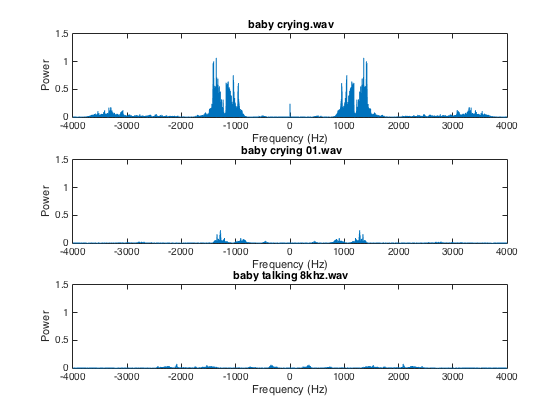
\includegraphics[width=1\textwidth]{sections/freq_spec_baby_linkaxis.png}
%  \caption{Frequency spectrum for baby sound files}
%  \label{fig:baby_spec}
%\end{figure}
%
%\begin{figure}[h]
%  \centering
%  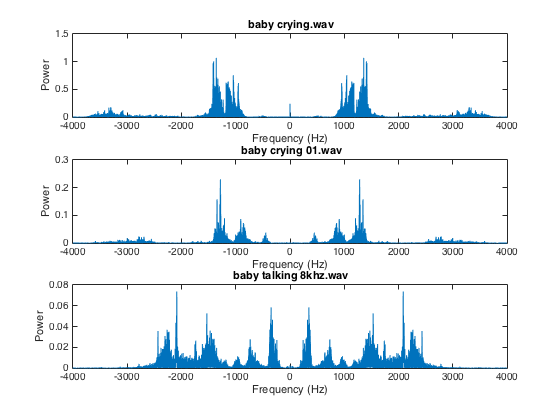
\includegraphics[width=1\textwidth]{sections/freq_spec_babyFix.png}
%  \caption{Frequency spectrum for baby sound files with scaled y-axis}
%  \label{fig:enhanced}
%\end{figure}

\begin{figure}[!hp]
  \centering
  \begin{minipage}[b]{0.4\textwidth}
    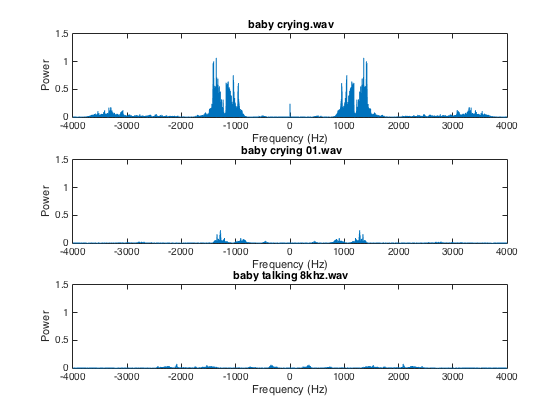
\includegraphics[width=1\textwidth]{sections/freq_spec_baby_linkaxis.png}
    \caption{Frequency spectrum for baby sound}
    \label{fig:baby_spec}
  \end{minipage}
  \hfill
  \begin{minipage}[b]{0.4\textwidth}
    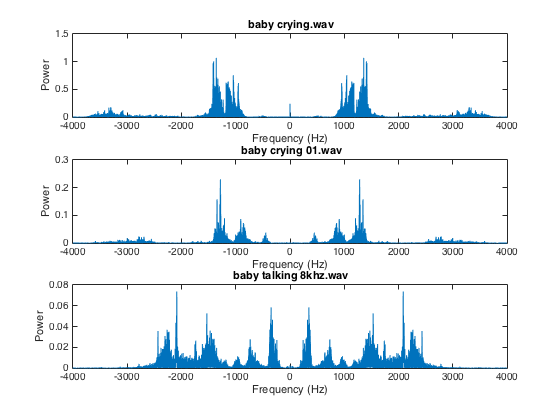
\includegraphics[width=1\textwidth]{sections/freq_spec_babyFix.png}
    \caption{Frequency spectrum for baby sound, scaled y-axis}
    \label{fig:enhanced}
  \end{minipage}
\end{figure}

\begin{figure}
  \centering
  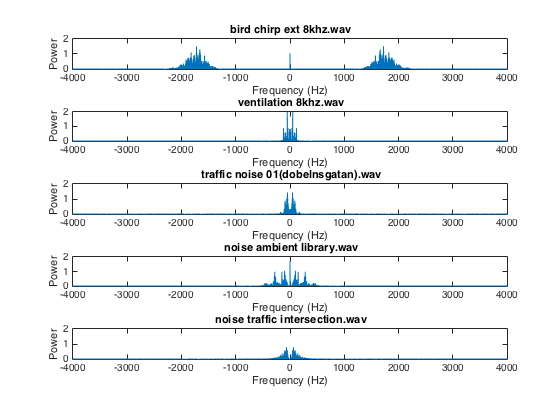
\includegraphics[width=1\textwidth]{sections/freq_spec_noise_2.png}
  \caption{Frequency spectrum for noise files}
  \label{fig:noise_spec}
\end{figure}

A quick and simple way to implement a BAD algorithm is to measure the power from the input signal.
Mathematically described, the power equation is given by the following formula: 
\[
P(n) = \frac{1}{N} \sum\limits_{k=0}^{N-1} x^2(n-k)
\]
where $P(n)$ is a vector. Since the BAD application is calculating the power of the input signal in 
real-time, this equation becomes impossible to implement. Hence, the usage of the \emph{recursive
averaging} algorithm. It is, in perspective to memory usage, a light and hardware friendly algorithm 
that calculates the average power level of the signal. Given the equation below,
\[
P(n) = \alpha P(n-1)+(1-\alpha)x^2(n)
\]
instead of performing the calculation for one sample at the time, a block of samples (simulating an interval) are calculated and summed.
The old result is saved to be used as $P(n-1)$. The $\alpha$ is a constant between 0 and 1 and is related to the 
following formula:
\[
\alpha = \frac{1}{T_{s}F_{s}}
\]
Despite that the $\alpha$ can be calculated, the get the best results further tweaking and testing is required.
For this BAD algorithm an $\alpha$ value of $0.5$ was choosen as the new value should be equaly summed by the old and
new power calculation.

The advanced algorithm is based upon the on the same, \emph{recursive averaging}, algorithm but before calculating
the average power the signal is first filtered through a Butterworth bandpass filter to remove unwanted 
frequencies. With the noise frequencies suppressed, the average power will focus on baby sound frequencies only. 

\begin{figure}{hp}
  \centering
  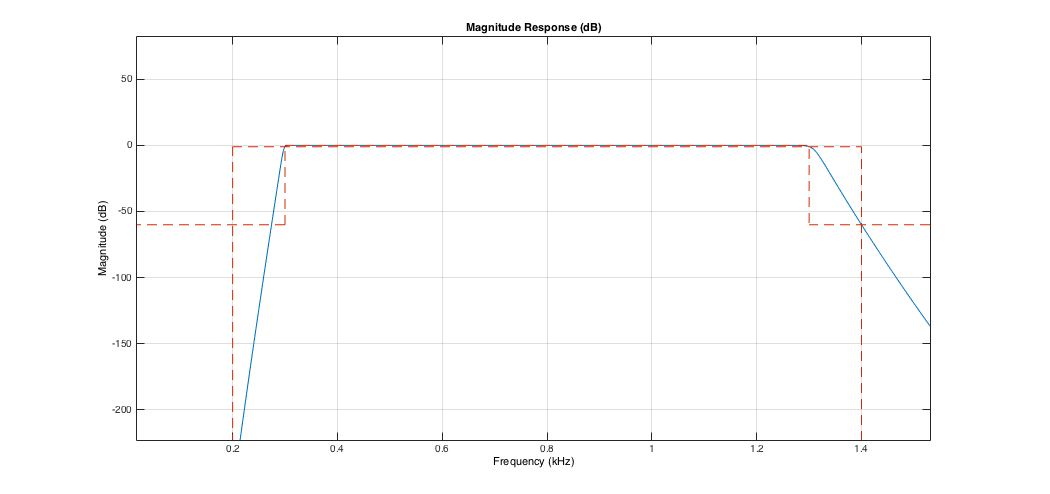
\includegraphics[width=1\textwidth]{sections/butt_pass_scale.png}
  \caption{Butterworth 300-1300 Hz bandpass filter}
  \label{fig:butt_pass}
\end{figure}

